\documentclass[11pt,a4paper]{article}

\usepackage[utf8]{inputenc}
\usepackage[T1]{fontenc}
\usepackage[spanish,es-tabla,es-nodecimaldot]{babel}
\usepackage{lmodern}
\usepackage{microtype}
\usepackage[margin=2.5cm]{geometry}
\usepackage{amsmath,amssymb}
\usepackage{graphicx}
\usepackage{booktabs}
\usepackage{tabularx}
\usepackage{array}
\usepackage{xcolor}
\usepackage{enumitem}
\usepackage{caption}
\usepackage{float}
\usepackage[hidelinks]{hyperref}

\graphicspath{{../img/}}
\setlist{itemsep=2pt,topsep=4pt}
\captionsetup{font=small,labelfont=bf}
\newcommand{\code}[1]{\texttt{#1}}
\newcommand{\SI}[2]{#1\,#2}  % cantidad con unidad (sin depender de siunitx)
\newcommand{\best}[1]{\textbf{#1}}

\title{\textbf{Robot de auto-balanceo de dos ruedas con aprendizaje por refuerzo profundo}\\[4pt]
\large Informe final --- CC3104 Aprendizaje por Refuerzo}
\author{Christian Echeverría \and Mario Betancourt\\[2pt]
\small Universidad del Valle de Guatemala\\[2pt]
\small Repositorio: \url{https://github.com/Ctribsz/ProyectoFinal-APR}}
\date{9 de noviembre de 2026}

\begin{document}
\maketitle

\begin{abstract}
Se comparan cuatro algoritmos de control continuo de Stable-Baselines3 (DDPG, TD3, SAC y PPO) en la tarea de balancear un robot de dos ruedas simulado en MuJoCo, y se contrastan con un controlador PID en cascada. Los cuatro algoritmos se afinaron con el mismo presupuesto (40 pruebas de Optuna de 200\,000 pasos) y se entrenaron con un millón de pasos en un entorno con comandos de velocidad y empujones, con 10 semillas cada uno. Después se evaluaron en cuatro niveles de dificultad, en una prueba de empujón y entrenando con aleatorización de dominio. TD3 obtiene el mejor desempeño en las condiciones de entrenamiento (IQM del retorno 891 de 1000) y se recupera más rápido de los empujones. SAC es el más eficiente en muestras y el más consistente entre semillas. PPO es el que mejor generaliza, sin haberlo entrenado ahí, al nivel con ruido de sensores, latencia y física aleatorizada. Los diagnósticos internos confirman el mecanismo que distingue a TD3 de DDPG: DDPG sobreestima el valor $Q$ en unos 41 puntos de retorno, mientras que el doble crítico de TD3 lo subestima. Todos los agentes superan al PID cuando hay ruido y latencia, aunque el PID tolera empujones aislados más fuertes.
\end{abstract}

\section{Pregunta de investigación e hipótesis}

\begin{quote}
¿Qué algoritmo ofrece el mejor desempeño para el auto-balanceo robusto ante perturbaciones, y qué mecanismos técnicos de cada algoritmo explican ese resultado?
\end{quote}

Para que la comparación no se reduzca a entrenar cuatro veces con valores por defecto, el proyecto usa un entorno propio con dificultad creciente, el mismo presupuesto de afinamiento y de pasos para todos los algoritmos, varias semillas con estadística robusta, diagnósticos internos que explican los resultados, y una línea base clásica. Las hipótesis se escribieron antes de los experimentos finales:
\begin{description}[font=\normalfont\bfseries]
  \item[H1] TD3 sobreestima menos $Q$ que DDPG y por eso entrena de forma más estable.
  \item[H2] SAC se recupera mejor de empujones grandes, por la exploración que le da la entropía.
  \item[H3] PPO necesita más pasos de entorno, pero tiene menor varianza entre semillas.
  \item[H4] Los agentes igualan al PID en el nivel 0 y lo superan en los niveles 2 y 3.
\end{description}

\section{Entorno}

\subsection{Modelo físico}

El robot se modela en MJCF como un chasis de \SI{1.0}{kg} y \SI{0.30}{m} de alto que pivota sobre dos ruedas de \SI{4}{cm} de radio separadas \SI{18}{cm}, con un motor de hasta \SI{0.3}{N\,m} por rueda. La física corre a \SI{500}{Hz} y el control a \SI{100}{Hz}. Los sensores imitan a un robot real: una IMU (orientación, giroscopio con saturación en $\pm$\SI{2000}{°/s} y acelerómetro) y encoders en las ruedas.

\subsection{Observación, acción y recompensa}

La observación tiene nueve valores y solo usa lo que mediría un robot real (tabla~\ref{tab:obs}); nunca la posición absoluta ni el estado interno del simulador.

\begin{table}[H]
\centering
\caption{Espacio de observación.}
\label{tab:obs}
\begin{tabular}{@{}cll@{}}
\toprule
Índice & Variable & Fuente equivalente \\
\midrule
0 & Pitch $\theta$ & IMU \\
1--2 & Velocidad de pitch $\dot\theta$ y de giro $\dot\psi$ & Giroscopio \\
3--4 & Velocidad de cada rueda & Encoders \\
5--6 & Comandos $v^*$ y $\dot\psi^*$ & Comando externo \\
7--8 & Acción anterior & Memoria del controlador \\
\bottomrule
\end{tabular}
\end{table}

La acción es un comando normalizado $a\in[-1,1]^2$, uno por motor. La recompensa por paso es una suma ponderada de componentes, que se registran por separado:
\begin{equation}
r_t = w_\text{alive} - w_\theta\,\theta^2 - w_{\dot\theta}\,\dot\theta^2 - w_v (v-v^*)^2 - w_{\dot\psi}(\dot\psi-\dot\psi^*)^2 - w_\text{effort}\lVert a_t\rVert^2 - w_\text{smooth}\lVert a_t-a_{t-1}\rVert^2 .
\end{equation}
El episodio termina si $|\theta|>0.6$\,rad (el robot cayó) y se trunca a los 1000 pasos (\SI{10}{s}). El retorno máximo es 1000.

\subsection{Niveles de dificultad}

\begin{table}[H]
\centering
\caption{Niveles de dificultad. Todos comparten el espacio de observación: se entrena en uno y se evalúa en todos.}
\label{tab:niveles}
\begin{tabularx}{\textwidth}{@{}cX@{}}
\toprule
Nivel & Qué agrega \\
\midrule
0 & Balanceo en reposo. \\
1 & Empujones aleatorios de hasta \SI{8}{N} durante \SI{0.1}{s}, uno cada \SI{2}{s} en promedio, en la parte alta del chasis. \\
2 & Comandos de velocidad ($\pm$\SI{0.5}{m/s}) y de giro ($\pm$\SI{1}{rad/s}) que cambian cada 2--\SI{4}{s}. \textbf{Nivel de entrenamiento.} \\
3 & Ruido gaussiano en los sensores, latencia de 0--\SI{20}{ms}, masa $\pm$20\,\%, fricción $\pm$30\,\% y torque $\pm$10\,\%. La recompensa usa las lecturas limpias. \\
\bottomrule
\end{tabularx}
\end{table}

\subsection{Línea base: PID en cascada}

Un lazo externo convierte el error de velocidad en un pitch objetivo, un lazo interno convierte el error de pitch en torque, y un término diferencial entre ruedas controla el giro. El PID usa solo la observación, igual que los agentes, y se evalúa con el mismo código. Sus ganancias se eligieron con una búsqueda en rejilla en el nivel 0. El lazo de velocidad tiene que ser lento: para frenar, el robot primero acelera las ruedas (fase no mínima), y con ganancias altas se vuelve inestable.

\section{Método}

\subsection{Pipeline común}

Los cuatro algoritmos pasan por los mismos scripts de entrenamiento, afinamiento y evaluación (\code{training/train.py}, \code{training/tune.py}, \code{evaluation/}), y solo cambia el archivo YAML de cada uno. La red es fija para todos: una MLP $[256,256]$. Cada corrida guarda la semilla, la configuración completa, las versiones de las librerías, el commit de git, la máquina y la duración. El repositorio tiene 112 pruebas automáticas.

\subsection{Afinamiento}

Cada algoritmo se afinó con Optuna en el nivel 2, con el mismo presupuesto: 40 pruebas de 200\,000 pasos, muestreador TPE y poda por mediana. El objetivo es la media de las últimas tres evaluaciones. Se afinaron los hiperparámetros que la literatura señala como críticos para cada algoritmo (tabla~\ref{tab:afinamiento}).

\begin{table}[H]
\centering
\caption{Mejor configuración encontrada por algoritmo (40 pruebas $\times$ 200\,000 pasos, nivel 2).}
\label{tab:afinamiento}
\small
\begin{tabularx}{\textwidth}{@{}lcX@{}}
\toprule
Algoritmo & Objetivo & Hiperparámetros elegidos \\
\midrule
DDPG & 836.3 & lr $8.85\times10^{-4}$, ruido de exploración $\sigma=0.236$, $\tau=0.0171$, batch 256 \\
TD3 & 896.9 & lr $1.95\times10^{-3}$, ruido de la política objetivo 0.448, retraso de la política 4, $\sigma=0.478$ \\
SAC & 878.1 & lr $2.29\times10^{-4}$, coeficiente de entropía automático, $\tau=0.0055$, batch 128 \\
PPO & 865.9 & lr $1.61\times10^{-4}$, clip 0.163, 16 épocas, 2048 pasos por rollout, $\lambda=0.950$ \\
\bottomrule
\end{tabularx}
\end{table}

\subsection{Protocolo experimental}

Con la mejor configuración, cada algoritmo se entrenó un millón de pasos en el nivel 2 con 10 semillas, y en el nivel 3 con 5 semillas (experimento E5). La evaluación final usa la política determinista, 50 episodios por nivel con semillas fijas, distintas de las de entrenamiento e iguales para todas las políticas. Entre semillas se reporta el IQM (media intercuartil) con intervalos de confianza al 95\,\% por bootstrap. La tabla~\ref{tab:experimentos} resume los experimentos.

\begin{table}[H]
\centering
\caption{Experimentos.}
\label{tab:experimentos}
\small
\begin{tabularx}{\textwidth}{@{}clX@{}}
\toprule
Id & Experimento & Pregunta \\
\midrule
E1 & Curvas por pasos de entorno & ¿Quién aprende con menos interacción? \\
E2 & Curvas por tiempo de reloj & ¿Quién aprende más rápido en la práctica? \\
E3 & Desempeño final en los niveles 0--3 & ¿Quién generaliza a condiciones más duras? \\
E4 & Prueba de empujón & ¿Cuánta fuerza tolera cada uno y qué tan rápido se recupera? \\
E5 & Entrenar con aleatorización (nivel 3) & ¿La aleatorización mejora la robustez? \\
E6 & Comparación contra el PID & ¿Dónde aporta el RL frente al control clásico? \\
\bottomrule
\end{tabularx}
\end{table}

\section{Resultados}

\subsection{E1 y E2: eficiencia de muestras y de tiempo}

\begin{figure}[H]
\centering
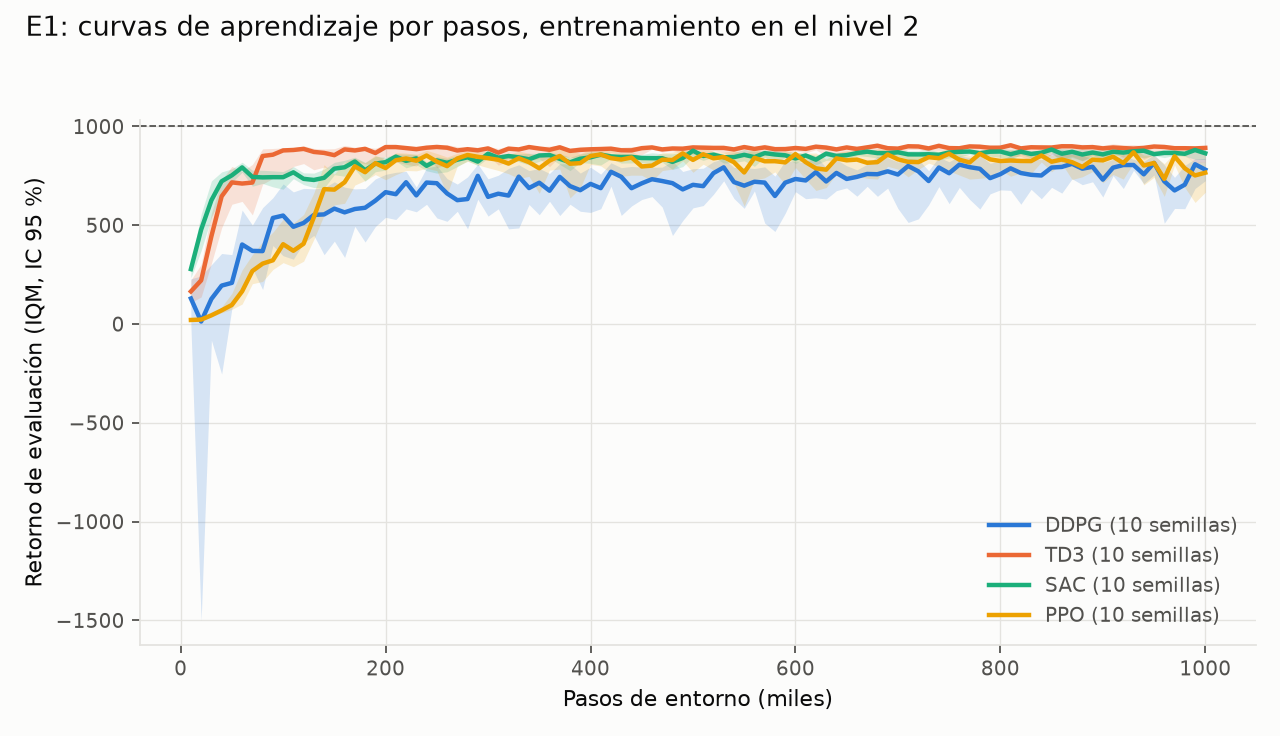
\includegraphics[width=\textwidth]{finales_level2_pasos.png}
\caption{Retorno de evaluación durante el entrenamiento en el nivel 2 (IQM de 10 semillas e IC 95\,\%).}
\label{fig:e1}
\end{figure}

\begin{table}[H]
\centering
\caption{Desempeño al final del entrenamiento en el nivel 2 (10 semillas). Retorno final: media de las últimas 3 evaluaciones de cada corrida. Las horas se miden en la máquina donde corrió cada algoritmo (laptop i7 de 4 núcleos o Ryzen 7 de 8; las 3 semillas de DDPG en Colab no cuentan).}
\label{tab:e1}
\small
\begin{tabular}{@{}lccccc@{}}
\toprule
Algoritmo & IQM del retorno final & Peor / mejor & Pasos al 90\,\% & Horas al 90\,\% & Máquina \\
\midrule
DDPG & 756.5 [674.5, 809.6] & 511 / 871 & 175k & 1.43 & laptop \\
TD3 & \best{891.1} [832.7, 897.8] & 572 / 907 & 75k & 0.27 & Ryzen 7 \\
SAC & 861.3 [844.7, 876.2] & \best{821} / 885 & \best{50k} & 0.43 & Ryzen 7 \\
PPO & 767.1 [678.5, 813.2] & 410 / 856 & 145k & 0.28 & laptop \\
\bottomrule
\end{tabular}
\end{table}

\begin{itemize}
  \item \textbf{TD3 llega al mejor desempeño} y se mantiene estable durante todo el entrenamiento (figura~\ref{fig:e1}).
  \item \textbf{SAC es el más eficiente en muestras} (90\,\% de su retorno final en 50\,000 pasos) y el más consistente: su peor semilla da 821 y su intervalo es el más angosto.
  \item \textbf{DDPG es el más lento e inestable}, con caídas bruscas en las curvas y la peor semilla en 511.
  \item \textbf{E2:} el tiempo de reloj solo se compara dentro de una misma máquina. En la laptop, PPO llega al 90\,\% en 0.28\,h y DDPG en 1.43\,h: aunque PPO necesita más pasos que TD3 o SAC, cada paso le cuesta unas 4 veces menos, porque hace muchas menos actualizaciones de gradiente por paso de entorno. En el Ryzen, TD3 (0.27\,h) es más rápido que SAC (0.43\,h). DDPG 4--6 corrieron en Colab y no entran en esta comparación.
\end{itemize}

\subsection{E3 y E6: generalización a los niveles 0--3 y comparación con el PID}

\begin{table}[H]
\centering
\caption{Retorno y tasa de caídas al evaluar en cada nivel a los agentes entrenados en el nivel 2 (IQM de 10 semillas, 50 episodios por nivel). El PID es determinista: se reporta su media.}
\label{tab:e3}
\small
\begin{tabular}{@{}clccccc@{}}
\toprule
Nivel & & DDPG & TD3 & SAC & PPO & PID \\
\midrule
0 & Retorno & 998 & 999 & \best{1000} & 994 & 999 \\
1 & Retorno & 947 & 975 & 958 & 924 & \best{995} \\
2 & Retorno & 748 & \best{891} & 854 & 769 & 807 \\
3 & Retorno & 283 & 374 & 257 & \best{537} & $-471$ \\
\midrule
1 & Caídas & 5\,\% & 1\,\% & 4\,\% & 14\,\% & \best{0\,\%} \\
2 & Caídas & 8\,\% & \best{0\,\%} & 2\,\% & 16\,\% & \best{0\,\%} \\
3 & Caídas & 51\,\% & \best{36\,\%} & 60\,\% & 39\,\% & 72\,\% \\
\bottomrule
\end{tabular}
\end{table}

\begin{table}[H]
\centering
\caption{Seguimiento de comandos y suavidad de las acciones, agentes entrenados en el nivel 2 (IQM).}
\label{tab:seguimiento}
\small
\begin{tabular}{@{}lccccc@{}}
\toprule
 & DDPG & TD3 & SAC & PPO & PID \\
\midrule
RMSE $v$, nivel 2 (m/s) & 0.496 & \best{0.350} & 0.404 & 0.479 & 0.545 \\
RMSE $v$, nivel 3 (m/s) & 0.632 & \best{0.550} & 0.667 & 0.580 & 1.522 \\
RMSE $\dot\psi$, nivel 2 (rad/s) & 0.459 & 0.226 & 0.232 & 0.310 & \best{0.123} \\
RMSE $\dot\psi$, nivel 3 (rad/s) & 1.281 & 0.891 & 1.134 & \best{0.475} & 2.954 \\
$\lVert a_t-a_{t-1}\rVert$, nivel 3 & 0.472 & 0.464 & 0.488 & \best{0.183} & 0.314 \\
Esfuerzo $\lVert a\rVert^2$, nivel 3 & 0.457 & 0.567 & 0.704 & \best{0.135} & 1.180 \\
\bottomrule
\end{tabular}
\end{table}

\begin{itemize}
  \item En el nivel de entrenamiento (2), \textbf{TD3 y SAC superan al PID}; DDPG y PPO quedan ligeramente por debajo, aunque siguen mejor la velocidad que el PID.
  \item En los niveles 0 y 1, sin comandos, el PID es tan bueno o mejor que los agentes: es el escenario para el que se ajustó.
  \item \textbf{En el nivel 3, todos los agentes superan con claridad al PID}, que cae en el 72\,\% de los episodios. Ningún agente vio ruido ni latencia durante su entrenamiento.
  \item \textbf{PPO es el que mejor generaliza al nivel 3}: el mejor retorno, el mejor seguimiento del giro y acciones mucho más suaves (0.18 contra $\sim$0.47 de los métodos off-policy) y con menos esfuerzo. Los algoritmos off-policy aprenden políticas deterministas muy reactivas, que amplifican el ruido de los sensores; es el mismo mecanismo que hace fallar al PID, con ganancias altas en el ángulo.
\end{itemize}

\subsection{E4: prueba de empujón}

En el nivel 0 se aplica un único empujón a $t=\SI{2}{s}$ en la parte alta del chasis, hacia adelante y hacia atrás, desde cinco estados iniciales. La fuerza máxima tolerada se busca por bisección; el tiempo de recuperación es el tiempo hasta que $|\theta|<2°$ de forma sostenida durante \SI{0.5}{s}.

\begin{table}[H]
\centering
\caption{Prueba de empujón, agentes entrenados en el nivel 2 (IQM de 10 semillas e IC 95\,\%).}
\label{tab:e4}
\small
\begin{tabular}{@{}lccc@{}}
\toprule
Política & Fuerza máxima (N) & Recuperación a \SI{4}{N} (s) & Recuperación a \SI{8}{N} (s) \\
\midrule
DDPG & 10.5 [9.9, 12.0] & 0.96 [0.87, 1.29] & 1.45 [1.18, 1.72] \\
TD3 & 12.7 [11.2, 13.6] & \best{0.78} [0.69, 0.92] & \best{1.06} [0.98, 1.20] \\
SAC & 12.2 [11.7, 12.9] & 1.10 [0.91, 1.26] & 1.38 [1.27, 1.57] \\
PPO & 9.0 [8.5, 10.0] & 1.30 [1.16, 1.40] & 1.82 [1.70, 2.37] \\
PID & \best{17.2} & 2.58 & 3.35 \\
\bottomrule
\end{tabular}
\end{table}

El PID tolera la mayor fuerza aislada, pero tarda unas tres veces más en volver a la vertical, porque frena inclinándose de forma lenta y controlada. Los agentes recuperan la vertical en alrededor de un segundo, a cambio de un margen menor ante empujones extremos. TD3 es el mejor de los agentes en las dos métricas.

\subsection{E5: entrenar con aleatorización de dominio}

\begin{table}[H]
\centering
\caption{Efecto de entrenar en el nivel 3 (5 semillas por algoritmo) frente a entrenar en el nivel 2. Retorno IQM al evaluar en cada nivel; entre paréntesis, el valor del agente entrenado en el nivel 2.}
\label{tab:e5}
\small
\begin{tabular}{@{}lcccc@{}}
\toprule
Evaluado en & DDPG & TD3 & SAC & PPO \\
\midrule
Nivel 1 & 958 (947) & 878 (975) & 898 (958) & 691 (924) \\
Nivel 2 & 794 (748) & 718 (891) & 673 (854) & 513 (769) \\
Nivel 3 & \best{654} (283) & 623 (374) & 649 (257) & 479 (537) \\
Caídas en el nivel 3 & \best{19\,\%} (51\,\%) & 41\,\% (36\,\%) & 41\,\% (60\,\%) & 69\,\% (39\,\%) \\
Fuerza máxima (N) & 11.8 (10.5) & 8.8 (12.7) & 9.8 (12.2) & 6.6 (9.0) \\
\bottomrule
\end{tabular}
\end{table}

\begin{itemize}
  \item Entrenar con aleatorización \textbf{sube el retorno en el nivel 3 para DDPG, TD3 y SAC} (por ejemplo, DDPG pasa de 283 a 654 y de 51\,\% a 19\,\% de caídas).
  \item A cambio, la mayoría \textbf{empeora en los niveles sin ruido} y tolera empujones menores: aprende una política más conservadora. DDPG es la excepción: mejora en los niveles 1 a 3 y queda igual en el 0.
  \item \textbf{PPO no se beneficia}: entrenado en el nivel 3 rinde peor en todos los niveles, incluso en el 3. Con el mismo presupuesto de pasos, el ruido en las observaciones parece dificultar su estimación de ventajas on-policy.
  \item Con 5 semillas los intervalos son anchos (por ejemplo, TD3 en el nivel 3: [415, 682]), así que estas diferencias deben leerse como tendencias.
\end{itemize}

\subsection{Diagnósticos internos}

\begin{figure}[H]
\centering
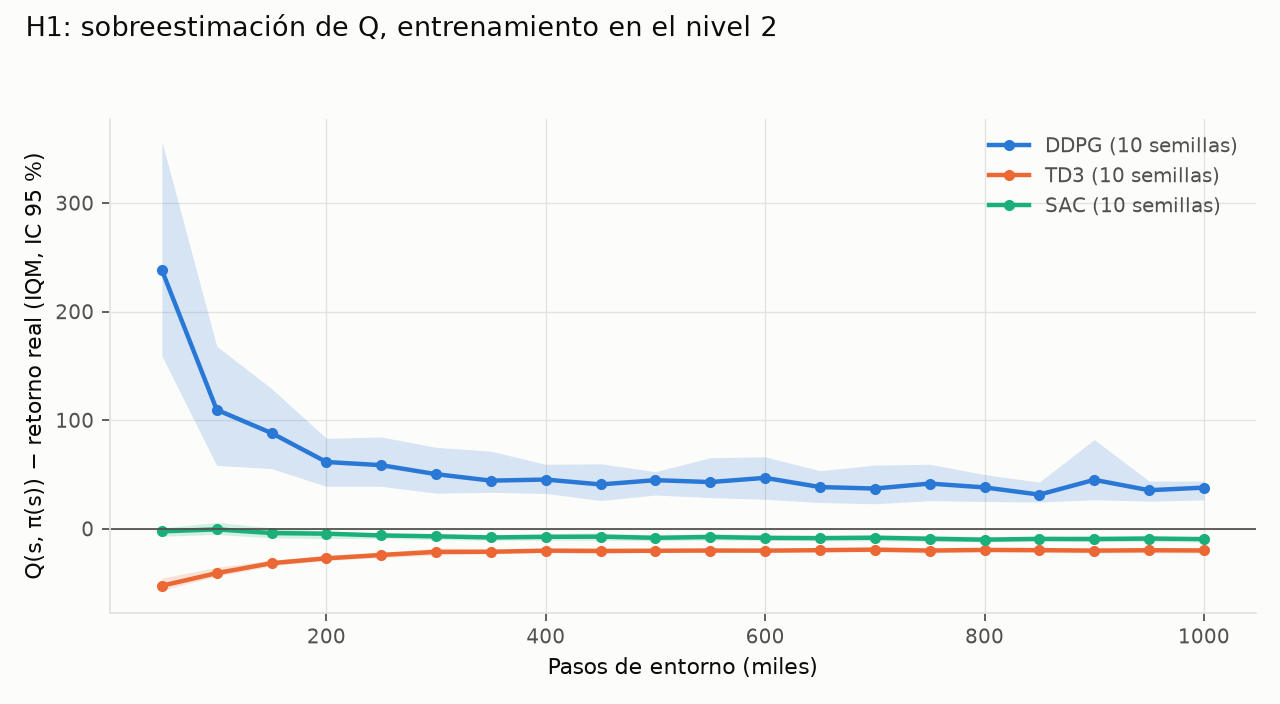
\includegraphics[width=0.85\textwidth]{finales_level2_q.png}
\caption{Sobreestimación de $Q$: diferencia entre $Q(s,\pi(s))$ del crítico y el retorno descontado real obtenido desde esos estados, cada 50\,000 pasos (IQM de 10 semillas).}
\label{fig:q}
\end{figure}

\begin{table}[H]
\centering
\caption{Diagnósticos al final del entrenamiento en el nivel 2 (media de los 3 últimos diagnósticos, IQM entre semillas).}
\label{tab:diag}
\small
\begin{tabular}{@{}lccc@{}}
\toprule
Algoritmo & Sobreestimación de $Q$ & $\lVert a_t-a_{t-1}\rVert$ & Energía de la acción $>$ \SI{5}{Hz} \\
\midrule
DDPG & $+41.0$ [28.3, 56.2] & 0.110 & 0.49 \\
TD3 & $-19.9$ [$-22.4$, $-18.1$] & 0.038 & 0.37 \\
SAC & $-9.1$ [$-11.9$, $-7.2$] & 0.041 & 0.44 \\
PPO & --- & 0.039 & \best{0.22} \\
\bottomrule
\end{tabular}
\end{table}

DDPG empieza sobreestimando $Q$ en más de 200 puntos y termina en $+41$ (figura~\ref{fig:q}). TD3, con el mínimo de dos críticos, subestima de forma estable ($-20$), y SAC, que también usa doble crítico pero suma el bono de entropía, queda cerca de cero. La sobreestimación de DDPG coincide con su entrenamiento más inestable y con acciones casi tres veces más bruscas.

\section{Contraste de hipótesis}

\begin{description}[font=\normalfont\bfseries]
  \item[H1 --- se confirma.] DDPG sobreestima $Q$ ($+41$) y TD3 no ($-20$), con intervalos que no se traslapan. TD3 entrena de forma más estable (peor semilla 572 contra 511, curvas sin caídas) y con acciones más suaves.
  \item[H2 --- se rechaza.] SAC no se recupera mejor que TD3: tolera una fuerza similar (12.2 contra \SI{12.7}{N}) y tarda más en recuperarse (1.38 contra \SI{1.06}{s} a \SI{8}{N}). La entropía le da consistencia entre semillas y eficiencia de muestras, pero no una mejor respuesta a los empujones.
  \item[H3 --- se confirma solo en parte.] PPO necesita más pasos que TD3 y SAC (145k contra 75k y 50k), pero menos que DDPG, y su varianza entre semillas no es menor: tiene la peor semilla (410) y uno de los intervalos más anchos. En tiempo de reloj, en cambio, es el más rápido.
  \item[H4 --- se confirma con matices.] Los cuatro agentes igualan al PID en el nivel 0 y lo superan con claridad en el nivel 3. En el nivel 2, solo TD3 y SAC lo superan en retorno, aunque los cuatro siguen mejor la velocidad. El PID conserva dos ventajas: no se cae en los niveles 1 y 2, y tolera el empujón aislado más fuerte.
\end{description}

\section{Limitaciones}

\begin{itemize}
  \item El afinamiento usa una sola semilla por prueba, así que la mejor configuración puede deberse en parte al azar. No hubo tiempo de revalidarla con más semillas.
  \item El nivel 3 tiene 5 semillas por algoritmo; sus intervalos son anchos.
  \item Las corridas se repartieron entre tres tipos de máquina (laptop, Ryzen 7 y Colab). El desempeño no depende de la máquina, pero el tiempo de reloj (E2) solo se compara dentro de cada una. DDPG 4--6 corrieron en Colab con Python 3.13; las demás librerías son iguales.
  \item \code{rliable.\allowbreak library} no funciona con pandas 3 en este entorno. El IQM sale de \code{rliable.metrics} y el bootstrap se implementó aparte con el mismo método (percentil, 95\,\%).
  \item No se normalizaron las observaciones: la prueba inicial con una semilla no fue concluyente y la decisión se aplicó igual a los cuatro algoritmos.
  \item El PID se ajustó en el nivel 0 y no se reajustó para el ruido del nivel 3. Un PID con filtros o ganancias más bajas probablemente reduciría su desventaja ahí.
\end{itemize}

\section{Conclusiones y dictamen}

\textbf{TD3 es el mejor algoritmo para esta tarea en las condiciones para las que se entrena}: tiene el mayor retorno, la menor tasa de caídas, el mejor seguimiento de velocidad y la recuperación más rápida ante empujones. El mecanismo que lo explica es el que predice H1: el doble crítico con el mínimo y el retraso de la política eliminan la sobreestimación de $Q$ que desestabiliza a DDPG.

\textbf{SAC es la alternativa más confiable}: queda cerca de TD3, aprende con menos muestras y casi no depende de la semilla.

\textbf{Si el robot va a operar con sensores ruidosos y latencia sin haberse entrenado para eso, PPO es la mejor opción}: produce acciones más suaves y con menos esfuerzo, que no amplifican el ruido. \textbf{Si se puede entrenar con aleatorización de dominio}, DDPG, TD3 y SAC recuperan esa robustez, y DDPG es el que más se beneficia.

Frente al control clásico, el aprendizaje por refuerzo aporta sobre todo robustez ante ruido y latencia, y mejor seguimiento de comandos. El PID sigue siendo competitivo en condiciones limpias y tolera mejor los empujones aislados muy fuertes.

\section*{Reparto del trabajo}

\begin{itemize}
  \item \textbf{Christian Echeverría:} modelo físico, entorno y niveles, PID, pipeline de entrenamiento, evaluación y prueba de empujón, TD3 y SAC (afinamiento y corridas finales).
  \item \textbf{Mario Betancourt:} DDPG y PPO (configuración, espacio de búsqueda, afinamiento y corridas finales), afinamiento con Optuna, diagnósticos internos, herramientas para correr en otras máquinas y en Colab, y el análisis estadístico de las corridas finales.
  \item \textbf{Ambos:} análisis, informe y dictamen.
\end{itemize}

\end{document}
